\documentclass[aspectratio=43]{beamer} % 16:9; drop for 4:3
\usetheme{Madrid} % try: Berkeley, CambridgeUS, metropolis (if installed)
\title{
  A Simple and Efficient Algorithm for Finding Minimum Spanning Tree Replacement Edges\\[1em]
}
\subtitle{
  David A. Bader, Paul Burkhardt\\
  {\footnotesize\url{http://jgaa.info/} vol.~26, no.~4, pp.~577-588 (2022)}  
}
\author{Bence Nagy}
\institute{ELTE IK}
\date{Gráfelméleti és optimalizálási módszerek, 2025}

\usepackage[utf8]{inputenc}
\usepackage[T1]{fontenc}
\usepackage[magyar]{babel}

\begin{document}

\begin{frame}
  \titlepage
\end{frame}

\section{Bevezetés}
\begin{frame}{Minimum feszítő fa + a feladat}
   \begin{columns}[c]
    \column{0.55\textwidth}
      \begin{itemize}
        \item Egy irányítatlan, súlyozott gráfon egy olyan fa, amely minden csúcsot összeköt, és a lehető legkevesebb összsúllyal.
        \item Célunk: a fából, ha kiesek bármelyik él, akkor keressük meg a legjobb csere élet.
        \item Alkalmazása: hálózati problémák
      \end{itemize}
    \column{0.4\textwidth}
      \begin{center}
        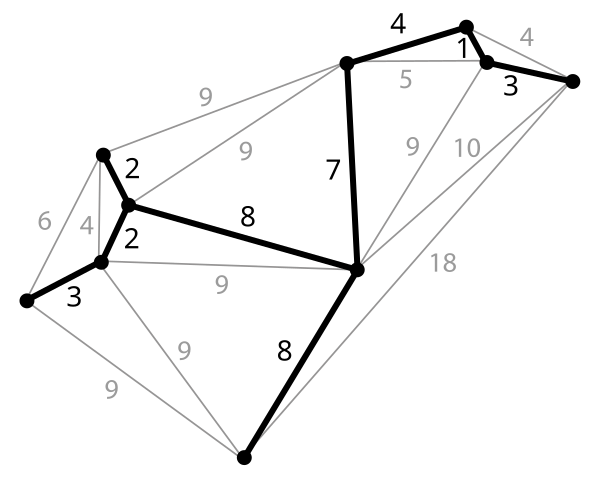
\includegraphics[width=\linewidth]{./images/MST_1.png}
      \end{center}
  \end{columns}
\end{frame}

\begin{frame}{}
  \begin{itemize}
    \item<1-> Első pont
    \item<2-> Második pont
    \item<3-> Harmadik pont
  \end{itemize}
\end{frame}

\begin{frame}{Képek és oszlopok}
  \begin{columns}
    \column{0.55\textwidth}
      \includegraphics[width=\linewidth]{example-image} % from mwe package
    \column{0.4\textwidth}
      \begin{block}{Megjegyzés}
      Rövid leírás a képről.
      \end{block}
  \end{columns}
\end{frame}

\end{document}
